\documentclass[12pt]{article}
\usepackage[a4paper, left=3.5cm, right=3.5cm, top=3.5cm, bottom=3.5cm, textwidth=12cm]{geometry}
\usepackage{setspace}
\setstretch{1,33}%20/12
\usepackage[english]{babel} 
\usepackage[utf8]{inputenc}
\usepackage{graphicx}
\usepackage[htt]{hyphenat}
\begin{document}

%
% ---- Titelseite ----
%
\begin{titlepage}
	\centering
	
\includegraphics[width=0.5\textwidth]{logo.png}\par\vspace{1cm}
	\vspace{1cm}
	{\scshape\Large CSCW and Groupware\par}
	\vspace{1.5cm}
	{\huge\bfseries Byzantine Fault Tolerance \par}
	\vspace{2cm}
	{\Large\itshape Lia Schulze Dephoff\par}
	{\itshape Study Program Informatik Master\par}
	{\itshape Matr.Nr. 375625\par}
	\vfill
	Dozent:\par
	Prof. Dr. \textsc{Prinz}

	\vfill

% Bottom of the page
	{\large \today\par}
\end{titlepage}

%
% ---- Inhaltsverzeichnis ----
%
\newpage
\tableofcontents 
\newpage
%
% ---- Einleitung ----
%
\section{Introduction}
Blockchains have become increasingly relevant since the introduction of the crypto currency Bitcoin in 2008 at the latest. Many companies are convinced of this technology and use it in various application areas. It is therefore particularly important that this system functions perfectly. A block chain is managed by a distributed network of computer nodes. In order for this system to function properly, the individual nodes must regularly communicate their current state and agree on a common consense. However, this common agreement can become complicated when faulty or dishonest nodes come into play. This problem is called the problem of the Byzantine generals. In the following, this problem is defined in more detail and the resulting principle of Byzantine fault tolerance is explained.

%
% ---- Hauptteil ----
%
\section{Byzantine Error}
A Byzantine error is a type of error in a network caused by a message being transmitted incorrectly. It can happen that the message is lost, but also that incorrect data is sent. This can be caused by an false state of a computer or by an incorrect response from the system.\cite{zyzzyva} Such types of errors are usually difficult to detect and therefore complicated to handle.\newline
To describe this kind of error in more detail, the problem of the Byzantine generals can be taken as an example.

\section{The problem of byzantine generals}
The problem of the Byzantine generals was posed in 1982 by Leslie Lamport, Robert Shostak and Marshall Pease and explained in the paper \glqq The Byzantine Generals Problem\grqq \cite{orig paper}.\newline
The problem describes the Byzantine army, which is divided into different divisions and besieges an enemy city. Each division has a general and there is no direct communication between them. The generals must now decide together whether to retreat or attack the city. To communicate with each other, a messenger is sent back and forth between them.
In the end, only a common agreement can lead to a successful plan, because the attack of only a few divisions would not lead to success.
The problem what arises from this is the lack of knowledge about whether all generals are loyal. There is a possibility that some generals are traitors and could try to prevent the agreement, so that in the end some of the divisions attack because they heard that this was the general decision, but others heard the opposite and retreat. This situation is illustrated again in Figure 1. The red figure is the traitor in this scenario. Because of his ambiguous messages to the other three generals, it happens that two of the four generals attack, one retreats and the traitor himself retreats as well. The decisions are simply made by a majority voting. Only the traitor does whatever he decides no matter what the voting resulted in. This leads to the situation that the two divisions try to attack the city alone, which most likely won't succeed.\newline
This problem can be transferred very well to blockchains, where the single nodes of the blockchain are seen as the generals and the connections between them are the messengers. As soon as a node is faulty or has fraudulent intentions, there is a risk that the system will not find a safe consensus. As a result, a participant could transmit incorrect transactions and thus destroy the effectiveness and reliability of the block chain.\cite{blockchainwelt}\newline

\begin{figure}[htbp] 
  \centering
     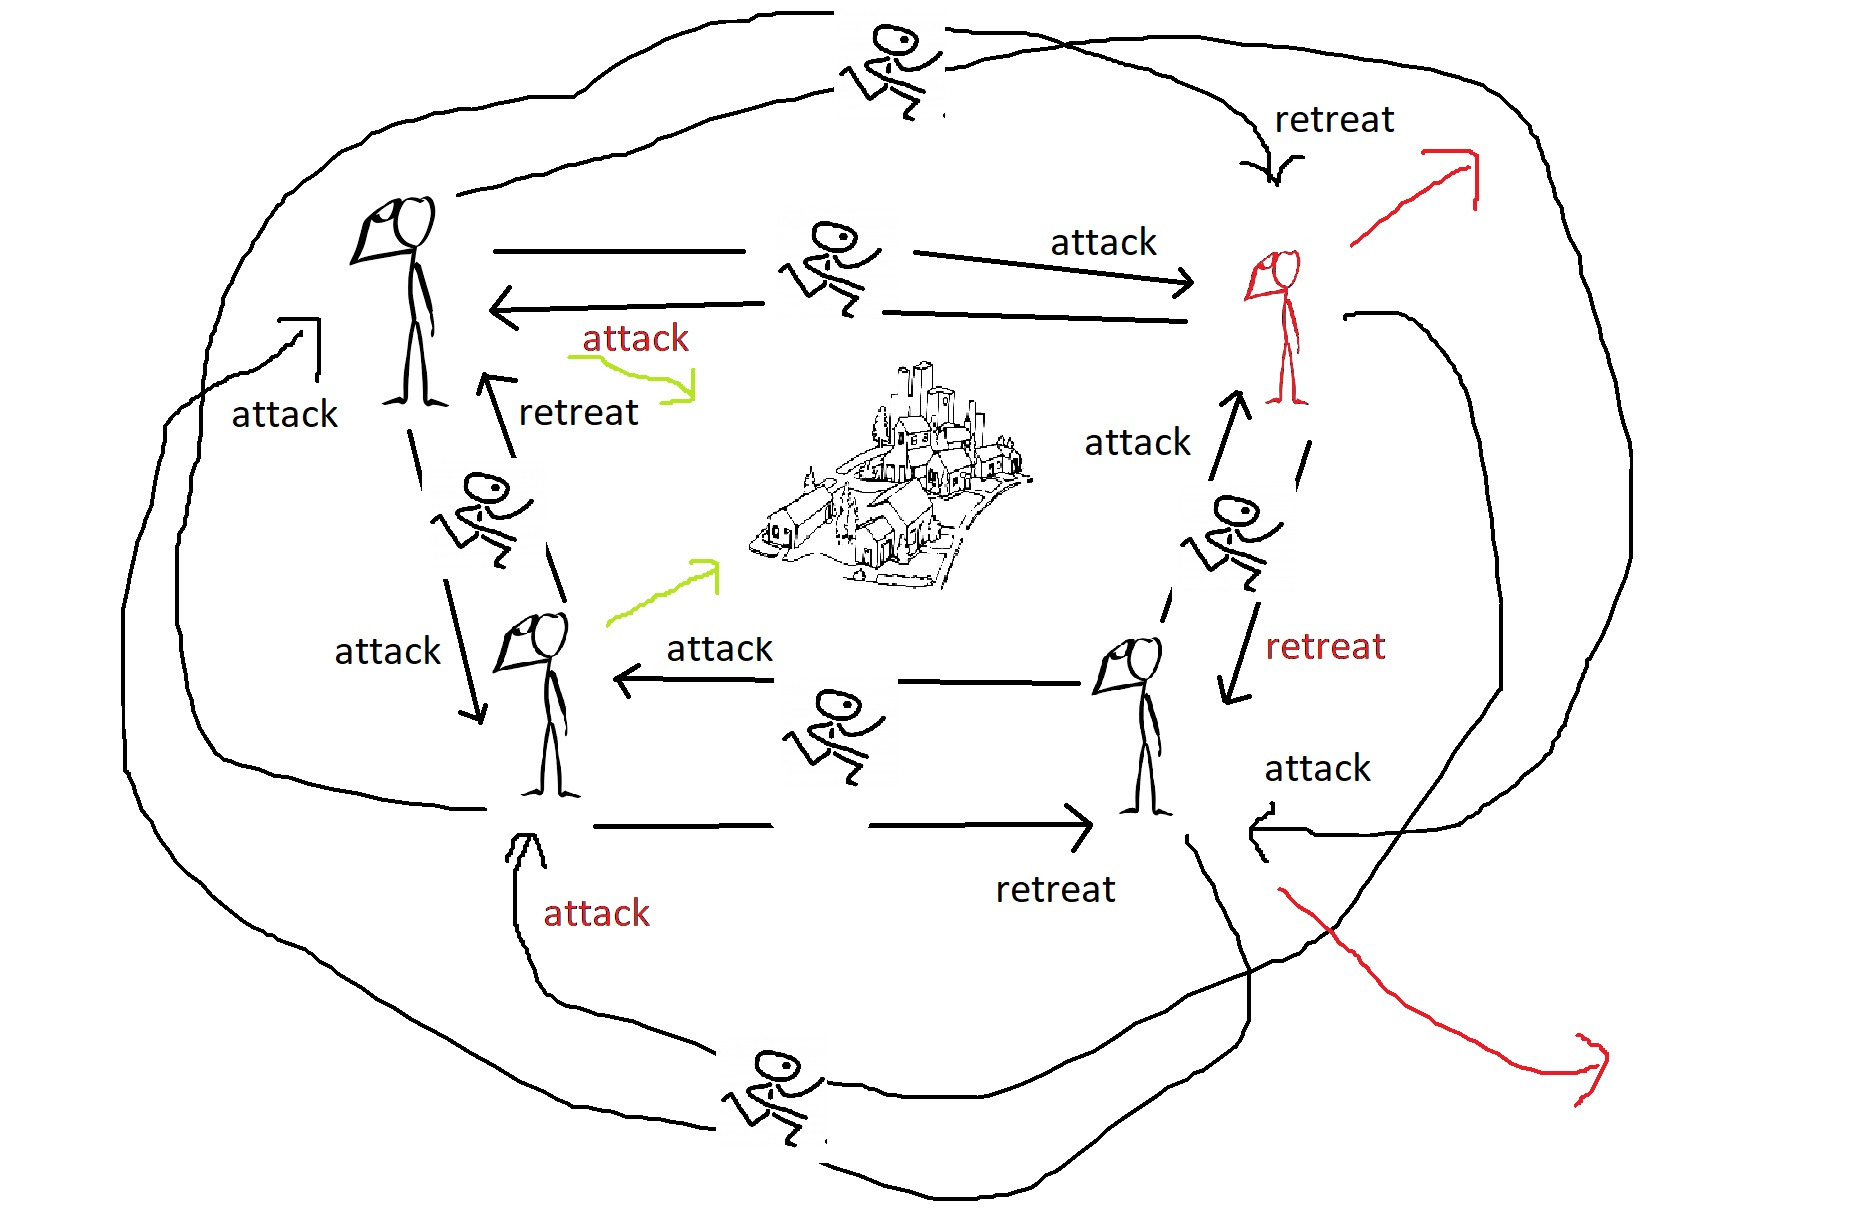
\includegraphics[width=1\textwidth]{byzantineProblem.jpg}
  \caption{Problem der byzantinischen Generäle}
  \label{fig:Bild1}
\end{figure}

\section{Commander-Lieutenant Problem}
In the paper by Leslie Lamport, Robert Shostak and Marshall Pease \cite{orig paper} 
the problem is reduced to the Commander Lieutenant Problem. This is about the fact that each commander has a group of lieutenants that he has to command, whether to attack or retreat. Again, the action of the lieutenants must be the same at the end for it to be successful. Under the condition that communication only works via messengers, more than two thirds of the generals must then be loyal in order to solve the problem. Otherwise it is not possible to recognize who is a traitor among the participants. In figure 2 you can see how the situation looks like reduced to one commander and two lieutenants. For Lieutenant 1, it is not possible to see which of the two participants is the traitor, because he receives the same orders in the upper situation with Lieutenant 2 as traitor and in the second situation with the commander as traitor. In this situation, Lieutenant 1 then has to attack and Lieutenant 2 has to retreat, because they have to obey the commanding officer's order and it is not possible to recognize whether the commander is a traitor or not.
So it can be shown that with a number of n generals and t traitors, the problem can only be solved if n\textgreater3t.
\begin{figure}[htbp] 
  \centering
     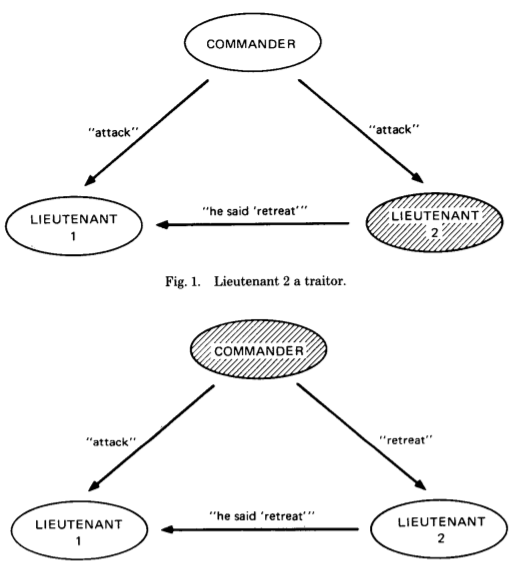
\includegraphics[width=0.5\textwidth]{commanderLeutnant.PNG}
  \caption{Commander-Lieutenant Problem}
  \label{fig:Bild2}
\end{figure}

\section{The Byzantine Fault Tolerance}
A system that overcomes the problem of the Byzantine generals is called Byzantine fault tolerant. If a Byzantine error occurs in the system, this system can therefore continue to work correctly. The system therefore tolerates this type of error.
Block chain systems like Bitcoin must surely have this kind of tolerance. However, there are other critical systems that must be protected against Byzantine errors. For example, airplanes and nuclear power plants are systems with a particularly high security risk.\cite{blockchainwelt}\newline
To achieve a Byzantine fault-tolerant system, there are several algorithms that try to solve this problem, so-called consensus algorithms. Probably the best known and best working algorithm at present is the Proof of Work algorithm, which is also used by Bitcoin. But even this algorithm does not promise a hundred percent protection against Byzantine errors, but is currently one of the safest options against Byzantine errors.\cite{binance academy}


%
% ---- Schlusswort ----
%
\section{Conclusion}
The Byzantine fault tolerance, is therefore the tolerance of a system against Byzantine errors. These are those that concern the problem of the Byzantine generals.
The problem of the Byzantine generals can be reduced to the commander-lieutenant problem, which shows that with more than two thirds of loyal generals the problem can be solved.\newline
To achieve this tolerance there are different algorithms that are used in Bitcoins, but also in airplanes or nuclear power plants.\newline
Byzantine fault tolerance is especially important in systems that require high security and promises security against system failures, as well as malicious nodes in the network. Even though the best, up-to-date algorithms cannot provide complete security against Byzantine errors, they are reliable and trustworthy.

%
% ---- Literatur ----
%
\begin{thebibliography}{5}
%

\bibitem {blockchainwelt}
Kai Schiller.
\textit{Was ist eine Byzantine Fault Tolerance (BFT)?}
\texttt{https://blockchainwelt.de/byzantine-fault-tolerance-bft-blockchain-algorithmus/}

\bibitem{zyzzyva}
Jonathan Koscielny.
\textit{Zyzzyva - Byzantinische Fehlertoleranz mit spekulativer Ausführung}\newline
Institut für Betriebssysteme und Rechnerverbund,Technische Universität Braunschweig

%\bibitem{Rampart}
%Frank Mattauch.
%\textit{Byzantinische Fehlertoleranz durch Gruppenkommunikation am Beispiel des %Rampart-Toolkit}\newline
%Friedrich-Alexander-Universität Erlangen-Nürnberg 

\bibitem{orig paper}
LESLIE LAMPORT, ROBERT SHOSTAK, and MARSHALL PEASE.
\textit{The Byzantine Generals Problem}\newline
SRI International, ACM Transactions on Programming Languages and Systems, Vol. 4, No. 3, July 1982. 

\bibitem{binance academy}
Byzantinische Fehlertoleranz\newline
\texttt{https://www.binance.vision/de/blockchain/byzantine-fault-tolerance-explained}

%\bibitem{medium}
%Georgios Konstantopoulos
%\textit{Understanding Blockchain Fundamentals, Part 1: Byzantine Fault %Tolerance}\newline
%\texttt{https://medium.com/loom-network/understanding-blockchain-fundamentals-part-1-by%zantine-fault-tolerance-245f46fe8419}

%\bibitem{proseminar}
%Esra Ünal, \textit{Seminararbeit Byzantinische Fehler}\newline
%Freie Universität Berlin, Institut für Informatik

\end{thebibliography}

\end{document}
